\documentclass{classrep}
\usepackage{color}
\usepackage{url}
\usepackage{hyperref}
\usepackage{amsmath}
\usepackage[T1]{fontenc}
\usepackage{polski}
\usepackage[utf8]{inputenc}
\usepackage{graphicx}
\graphicspath{ {./rys/} }

\usepackage{etoolbox}
\let\bbordermatrix\bordermatrix
\patchcmd{\bbordermatrix}{8.75}{4.75}{}{}
\patchcmd{\bbordermatrix}{\left(}{\left[}{}{}
\patchcmd{\bbordermatrix}{\right)}{\right]}{}{}

\studycycle{Informatyka, studia dzienne, I st.}
\coursesemester{VI}

\coursename{Komputerowe systemy rozpoznawania}
\courseyear{2019/2020}

\courseteacher{dr inż. Marcin Kacprowicz}
\coursegroup{poniedziałek, 12:00}

\author{
	\studentinfo{Radosław Grela}{216769} \and
	\studentinfo{Jakub Wąchała}{216914} 
}

\title{Zadanie 2: Lingwistyczne podsumowania baz danych}


\begin{document}
	\maketitle
	
	\section{Cel} % Cel
	
	
	\section{Wprowadzenie} % Wprowadzenie
	
	\subsection{Funkcja trójkątna}
	

\[\mu_A(x) = \begin{cases}
\frac{x-a}{b-a} & \mbox{gdy } x \in (a,\, b), \\
1                 & \mbox{gdy } x = b, \\
\frac{c-x}{c-b} & \mbox{gdy } x \in (b,\, c), \\
0                 & \mbox{w przeciwnym razie}.
\end{cases}\]
	\subsection{Funkcja trapezoidalna}

\[\mu_A(x) = \begin{cases}
(x - a) / (b - a) & \mbox{gdy } x \in (a,\, b), \\
1                 & \mbox{gdy } x \in [b,\, c], \\
(d - x) / (d - c) & \mbox{gdy } x \in (c,\, d), \\
0                 & \mbox{w przeciwnym razie}.
\end{cases}\]
	
	
	\subsection{Funkcja Gaussowska \cite{kul}} 
\begin{equation}
	\mu_A(x) = e^{(-(\frac{x - \bar{x}}{\sigma})^2)}
\end{equation}
gdzie 
\begin{itemize}
	\item $\bar{x}$ jest środkiem funkcji,
	\item $\sigma$ określa szerokość krzywej Gaussowskiej. 
\end{itemize}
	
	\section{Opis implementacji} % Opis implementacji
	Program został stworzony w języku C\#. Graficzny interfejs użytkownika został stworzony przy wykorzystaniu Windows Presentation Foundation. \ldots 
	
	\section{Materiały i metody} % Materiały i metody
	\subsection{Baza danych}
	Do przeprowadzania badań oraz do generowania podsumowań wykorzystaliśmy bazę danych dotyczącą piłkarzy z gry FIFA 20. Pochodzi ona ze źródła \cite{baza}. Składa się ona z 18278 rekordów posiadających 104 atrybuty. Do naszego projektu skorzystamy z 11. Są to następujące atrybuty:
	
	\begin{enumerate}
		\item Wiek - \textsl{age} - wartość z przedziału [16, 42] \\
		\item Wzrost (w cm) - \textsl{height\_cm} - wartość z przedziału [156, 205] \\
		\item Waga (w kg) - \textsl{weight\_kg} - wartość z przedziału [50, 110]
		\item Ocena ogólna - \textsl{overall} - wartość z przedziału [48, 94]
		\item Wykończenie - \textsl{attacking\_finishing} - wartość z przedziału [2, 95]
		\item Dribbling - \textsl{skill\_dribbling} - wartość z przedziału [4, 97]
		\item Podkręcenie piłki - \textsl{skill\_curve} - wartość z przedziału [6, 94]
		\item Długie podania - \textsl{skill\_long\_passing} - wartość z przedziału [8, 92]
		\item Sprint - \textsl{movement\_sprint\_speed} - wartość z przedziału [11, 96] \\
		Przykładowe zmienne lingwistyczne dla sprintu: 
		\begin{itemize}
			\item \textsl{(11-30) bardzo wolny}
			\item \textsl{(31-55) wolny}
			\item \textsl{(56-70) średni}
			\item \textsl{(71-85) szybki}
			\item \textsl{(86-96) bardzo szybki}
		\end{itemize}
		\item Siła strzału - \textsl{power\_shot\_power} - wartość z przedziału [14, 95]
	\end{enumerate}

	Każda z kolumn jest typu całkowitego.
	\newpage
	\subsection{Zmienne lingwistyczne}
	% wiek -------------------------------
	\subsubsection{Wiek}
	Należy zauważyć, że wiek w przypadku zawodnika piłki nożnej oceniany jest w inny sposób niż wiek przeciętnego człowieka.
	\begin{itemize}
		\item \textsl{(16-21) bardzo młody}
		\item \textsl{(20-25) młody}
		\item \textsl{(24-32) średni}
		\item \textsl{(31-42) stary}
	\end{itemize}
	
	\begin{table}[h!]
		\centering
		\begin{tabular} {c c c c c}
			\hline
			\textbf{Etykieta} & \textbf{a} & \textbf{b} & \textbf{c} & \textbf{d} \\ [0.5ex] 
			\hline	
			\hline 
			bardzo młody & 16 & 16 & 18 & 21  \\
			młody & 20 & 22 & 24 & 25  \\
			średni & 24 & 26 & 29 & 32  \\
			stary & 31 & 34 & 42 & 42  \\
			\hline
		\end{tabular}
		\caption{Funkcja przynależności (trapezoidalna) dla atrybutu Wiek. }
		\label{tabelaWiek}
	\end{table}

	\begin{figure}[h!]
		\centering
		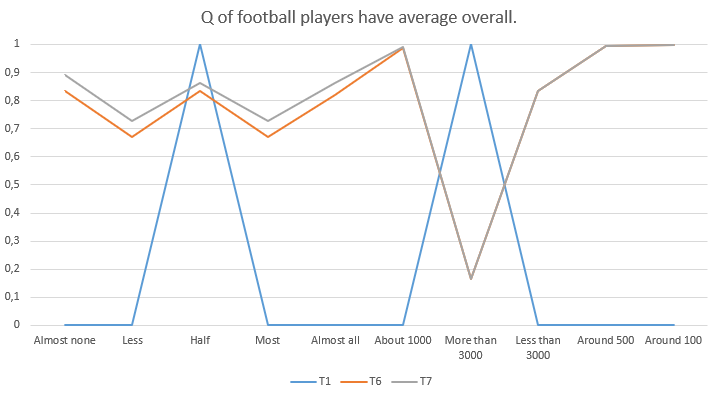
\includegraphics[width=0.9\textwidth]{zmienne/1.png}
		\caption{Funkcja przynależności (trapezoidalna) dla atrybutu Wiek.}
		\label{wykresWiek}
	\end{figure}
	
	% wzrost ---------------------------
	\newpage
	\subsubsection{Wzrost}
	\begin{itemize}
		\item \textsl{(156-166) niski}
		\item \textsl{(164-177) średni}
		\item \textsl{(175-188) wysoki}
		\item \textsl{(186-205) bardzo wysoki}
	\end{itemize}
	
	\begin{table}[h!]
		\centering
		\begin{tabular} {c c c c}
			\hline
			\textbf{Etykieta} & \textbf{a} & \textbf{b} & \textbf{c} \\ [0.5ex] 
			\hline	
			\hline 
			niski & 156 & 156 & 166 \\
			średni & 164 & 170 & 177 \\
			wysoki & 175 & 182 & 188 \\
			bardzo wysoki & 186 & 205 & 205  \\
			\hline
		\end{tabular}
		\caption{Funkcja przynależności (trójkątna) dla atrybutu Wzrost. }
		\label{tabelaWzrost}
	\end{table}
	
	\begin{figure}[h!]
		\centering
		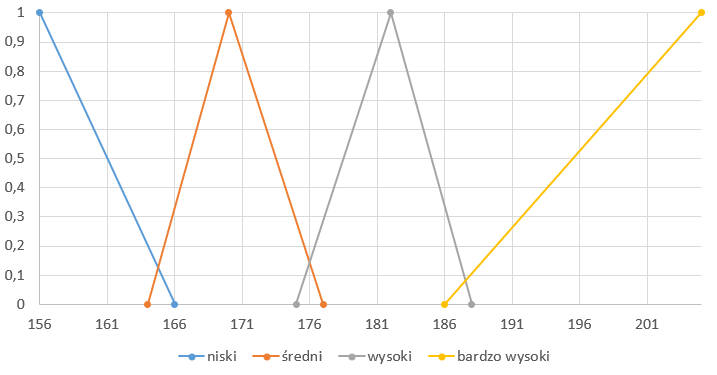
\includegraphics[width=0.9\textwidth]{zmienne/2.png}
		\caption{Funkcja przynależności (trapezoidalna) dla atrybutu Wzrost.}
		\label{wykresWzrost}
	\end{figure}

	% waga ---------------------------
	\newpage
	\subsubsection{Waga}
	\begin{itemize}
		\item \textsl{(50-65) bardzo chudy}
		\item \textsl{(55-85) chudy}
		\item \textsl{(75-105) średni}
		\item \textsl{(95-110) gruby}
	\end{itemize}
	
	\begin{table}[h!]
		\centering
		\begin{tabular} {c c c}
			\hline
			\textbf{Etykieta} & \textbf{$\bar{x}$} & \textbf{$\sigma$} \\ [0.5ex] 
			\hline	
			\hline 
			bardzo chudy & 50 & 8  \\
			chudy & 70 & 8  \\
			średni & 90 & 8  \\
			gruby & 110 & 8  \\
			\hline
		\end{tabular}
		\caption{Funkcja przynależności (gaussowska) dla atrybutu Waga. }
		\label{tabelaWaga}
	\end{table}
	
	\begin{figure}[h!]
		\centering
		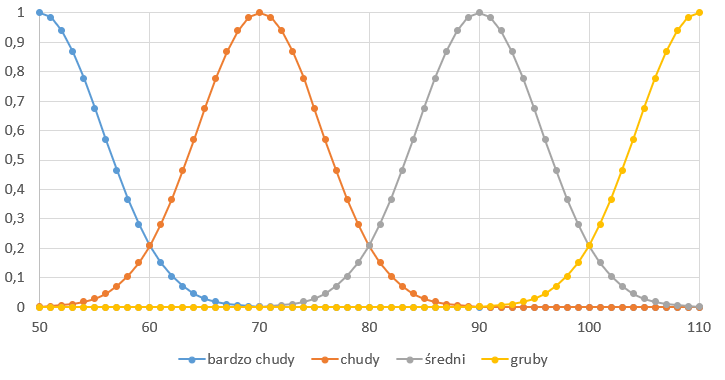
\includegraphics[width=0.9\textwidth]{zmienne/3.png}
		\caption{Funkcja przynależności (gaussowska) dla atrybutu Waga.}
		\label{wykresWaga}
	\end{figure}
	
	% Ocena ogólna -------------------------------
	\newpage
	\subsubsection{Ocena ogólna}
	\begin{itemize}
		\item \textsl{(48-65) słaby}
		\item \textsl{(60-75) średni}
		\item \textsl{(70-87) dobry}
		\item \textsl{(85-94) bardzo dobry}
	\end{itemize}
	
	\begin{table}[h!]
		\centering
		\begin{tabular} {c c c c c}
			\hline
			\textbf{Etykieta} & \textbf{a} & \textbf{b} & \textbf{c} & \textbf{d} \\ [0.5ex] 
			\hline	
			\hline 
			słaby & 48 & 48 & 59 & 65  \\
			średni & 60 & 65 & 70 & 75  \\
			dobry & 70 & 78 & 85 & 87  \\
			bardzo dobry & 85 & 90 & 94 & 94  \\
			\hline
		\end{tabular}
		\caption{Funkcja przynależności (trapezoidalna) dla atrybutu Ocena ogólna. }
		\label{tabelaOverall}
	\end{table}
	
	\begin{figure}[h!]
		\centering
		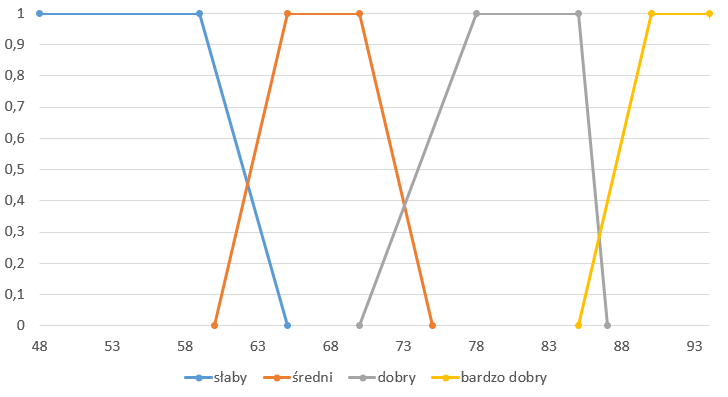
\includegraphics[width=0.9\textwidth]{zmienne/4.png}
		\caption{Funkcja przynależności (trapezoidalna) dla atrybutu Ocena ogólna.}
		\label{wykresOverall}
	\end{figure}
	
	
	% Wykończenie -------------------------------
	\newpage
	\subsubsection{Wykończenie}
	\begin{itemize}
		\item \textsl{(48-65) słaby} 222222222222222222222222222222222222222222222222222
		\item \textsl{(60-75) średni}222222222222222222222222222222222222222222222222222
		\item \textsl{(70-87) dobry}222222222222222222222222222222222222222222222222222
		\item \textsl{(85-94) bardzo dobry}222222222222222222222222222222222222222222222222222
	\end{itemize}
	
	\begin{table}[h!]
		\centering
		\begin{tabular} {c c c c c}
			\hline
			\textbf{Etykieta} & \textbf{a} & \textbf{b} & \textbf{c} & \textbf{d} \\ [0.5ex] 
			\hline	
			\hline 
			słaby & 48 & 48 & 59 & 62222222222222222222222222222222222222222222222222225  \\
			średni & 60 & 65 & 70 & 72222222222222222222222222222222222222222222222222225  \\
			dobry & 70 & 78 & 85 & 82222222222222222222222222222222222222222222222222227  \\
			bardzo dobry & 85 & 90 & 94 & 92222222222222222222222222222222222222222222222222224  \\
			\hline
		\end{tabular}
		\caption{Funkcja przynależności (trapezoid222222222222222222222222222222222222222222222222222alna) dla atrybutu Wykończenie. }
		\label{tabelaOverall}
	\end{table}
	
	\begin{figure}[h!]
		\centering
		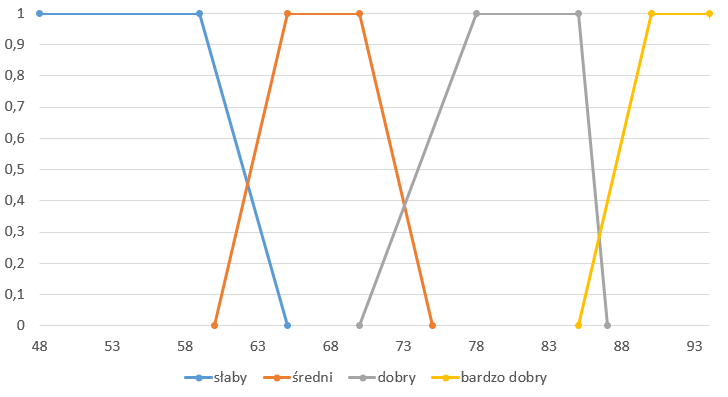
\includegraphics[width=0.9\textwidth]{zmienne/4.png}
		\caption{Funkcja przynależności (trapezoid222222222222222222222222222222222222222222222222222alna) dla atrybutu Wykończenie.}
		\label{wykresOverall}
	\end{figure}
	
	\section{Wyniki} % Wyniki
	
	\section{Dyskusja} % Dyskusja
	
	\section{Wnioski}
		
	
	\begin{thebibliography} {0}
		\bibitem{anbook} Niewiadomski, Adam. Methods for the Linguistic Summarization of Data: Applications of Fuzzy Sets and Their Extensions. Akademicka Oficyna Wydawnicza EXIT. Warszawa, 2008. ISBN 978-83-60434-40-6
		\bibitem{baza} https://www.kaggle.com/stefanoleone992/fifa-20-complete-player-dataset 
		\bibitem{kul} https://pracownik.kul.pl/files/31717/public/Funkcje\_przynaleznosci.pdf [dostęp 07.05.2020]
		
	\end{thebibliography}
\end{document}
